\section{General Aspects}
Ideally, every user could publish a document and that document could be discovered by any other users no matter where they are. However, the Internet poses some issues that make this ideal world hard to accomplish. In the following sections we will first analyze the fundamental problems we face when deploying a distributed application on the Internet and then propose some ways how one could deal with them.

\subsection{Firewalls/NAT}
Most Internet users today do not have public IP addresses. They are behind a NAT (network address translation) router and sometimes behind firewalls that they cannot control too (e.g. corporate users). If a user wants to publish a document, there must be some kind of server that accepts connections for the given document. If the server is behind a NAT router, there is usually no way an external client can connect to that document server. If the server is behind a firewall, the situation is even more problematic as the firewall will most likely block most incoming traffic. The basic dilemna with NAT routers and firewalls is depicted in figure \ref{fig:firewall}.

\begin{figure}[H]
 \centering
 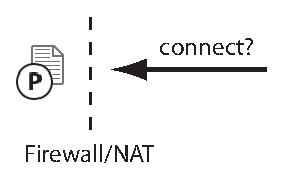
\includegraphics[width=4.2cm,height=2.6cm]{../../images/net_firewall.eps}
 \caption{Basic Problem with Firewalls and NAT Routers}
 \label{fig:firewall}
\end{figure}

\subsection{Tunneling Firewalls}
It would be possible to tunnel firewalls, although this technique is a bit delicate. Firewalls are there for a reason. Tunneling firewalls is most likely against the will of the security policy of a company. For this reason this is not considered to be a requirement for our application.

\subsection{Dealing with NAT Router}
The problem with NAT routers is, that nobody from the outside can connect to a computer on the inside because the computer on the inside does not have a public IP address. Of course it would be possible to set up the router in a way that it delegates requests for certain services to one particular computer, but we do not consider this as an acceptable technique for an end user application. We cannot expect end users to do this setup. The solution to this problem is, that first the client must establish a connection to a host outside of the local network. 

\subsubsection{Proxy Host}
Let us say there is a host $X$, called \emph{proxy}, and a host $A$, called \emph{publisher}. Host $A$ sits behind a NAT router and wants to publish a document. Host $A$ connects to the proxy host $X$ which publishes the document in stead of $A$. Every other client that wants to join the document published by $A$ connects to $X$. $X$ acts as a proxy and forwards all messages for that published document to $A$ (using the connection opened by host $A$). $X$ also forwards any responses/messages from $A$ to all the other clients of this editing session. This solution to the NAT problem is depicted by figure \ref{fig:proxy}.

\begin{figure}[H]
 \centering
 
\includegraphics[width=3.8cm,height=2.9cm]{../../images/net_proxy.eps}
 \caption{Proxy Host}
 \label{fig:proxy}
\end{figure}

\subsubsection{Substitute Host}
Let us say there is a host $X$, called \emph{substitute}, and a host $P$, called the publisher. Host $P$ again sits behind a NAT router and wants to publish a document. It connects to the substitute host $X$, which publishes the document and hosts the document itself. So host $P$ is no longer the publisher of the document, but merely an ordinary client. Host $X$ plays the substitute of host $P$ because he has a public IP address whereas host $P$ has not.

\begin{figure}[H]
 \centering
 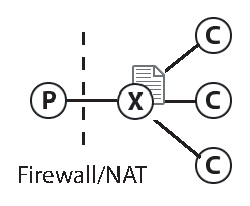
\includegraphics[width=3.7cm,height=2.9cm]{../../images/net_substitute.eps}
 \caption{Subsitute Host}
 \label{fig:substitute}
\end{figure}

The substitute host solution to the NAT problem is depicted by figure \ref{fig:substitute}. It is very similar to the proxy host solution. The only difference is, that the substitute host is itself the server whereas the proxy host is only a proxy forwarding all requests back to the publisher host $P$.


\subsection{Document Publishing}
When a user publishes a document, he wants other users to find it. There must be some kind of discovery mechanism that allows users to discover published documents. There are several solutions to this problem. 

On the LAN clients could use \emph{IP multicast} to discover documents (see section \ref{sect:jini} and section \ref{sect:bonjour}). IP multicast usually fails in WANs because routers block multicast traffic. A common and relatively straightforward solution for WANs would be to have a (or several load-balancing) \emph{central server} that manage all the document advertisements. A pure \emph{P2P solution} could build upon a P2P framework (see section \ref{sect:jxta}) to avoid central servers at all.
